%% in this chapter you are providing any background information that would be
%% needed by the reader to facilitate their comprehension of your thesis topic.
%% basically you need to provide knowledge that your intended audience may not
%% have.  in this case, your indended audience should be young researchers and
%% experienced researchers (yea it can be tough).  you should plan your writing
%% to target that the lowest academic level of your readership.  in particular
%% you writing should target graduate students approaching their second year of
%% graduate study.  also, you are not necessarily writing to all possible
%% graduate students; you can target the particular class of researchers that
%% would normally read something in this topic space.  remember you are
%% providing background to facilitate understanding; you do not need to explain
%% everything about each topic, just enough that they can develop a reasonably
%% clear understanding that will allow them to read and comprehend the research
%% project that your thesis encapsulates.

%% start with an introductory paragraph explaining what this chapter
%% contains.  answer the question: what background are you going to cover?

\chapter{Background}\label{bkgrnd}

The beginnings of computing machinery, up until the introduction of the von-Neumann architecture, were narrowly focused
on the ambition of mechanizing rote data processing and analysis work.  Although today we find ourselves in a
multifaceted computing landscape arguably not likely envisioned by computing's forefathers, data analysis still occupies
much of the computing research space.  Perhaps rightly so, as advances in data analysis have had a profound impact on
virtually every field of scientific, economic, and social interest.  While the computing performance has grown
exponentially over the years many principal problems remain unsolved.  One such problem is the statistical
classification problem, with the implied definition of identifying an observations classification as induced by other
observations.  Classes in the computing parlance are more commonly referred to as clusters, and likewise the
classification problem is often referred to as cluster analysis.  Principal among clustering problems is the $k$-means
clustering problem defined in MacQueen's 1967 paper ``Some methods for classification and analysis of multivariate
observations'' \cite{macqueen-67} boasting over 18,000 direct citations.

\section{$k$-Means Problem}

By restricting observations to a vector space, the clustering problem can be described as a partitioning problem in
which the goal is to optimize the demarcations bounds to group similar observations.  The $k$-means clustering problem
extends this definition to allow a user defined number of partitions, $k$ that are specified, to separate the
observations into $k$ distinct groups.  Extending this concept we get a simple heuristic for the performance of a
particular clustering.  Given a set of vectors $x\in X$ partition the data space into $k$ clusters $\{C_1, C_2, ...,
C_k\}$ of vectors such that the \emph{Within-Cluster Sum of Squares Error} (WCSSE) metric is minimized over all possible
partitioning.  More formally,
$$
{\underset{C}{\text{argmin}}} {\overset{k}{\underset{i=1}{\sum}}} {\underset{x\in C}{\sum}}
||x-\mu_i||^2, 
$$
where $\mu_i$ is the mean of the points in a partition or centroid of the cluster $C_i$. 

Figure \ref{kmex} displays an example of a standard $k$-means algorithm run on Gaussian data clusters with nine random
starting instances.  The above optimization is WCSSE statistic is given with each clustering attempt.  The example shows
the success of the WCSSE criterion in identifying the ground truths of a dataset while variability in correspondence
between estimated centroid partitions and ground data points demonstrates a key drawback of hard margin data clustering.
In \textsf{RPHash}, a focus on high clusters in high dimensional space, minimizes the risk of overlap, discussed more formally in
the section on occultation (Section \ref{occultationSection}).

\begin{figure}
    \centerline{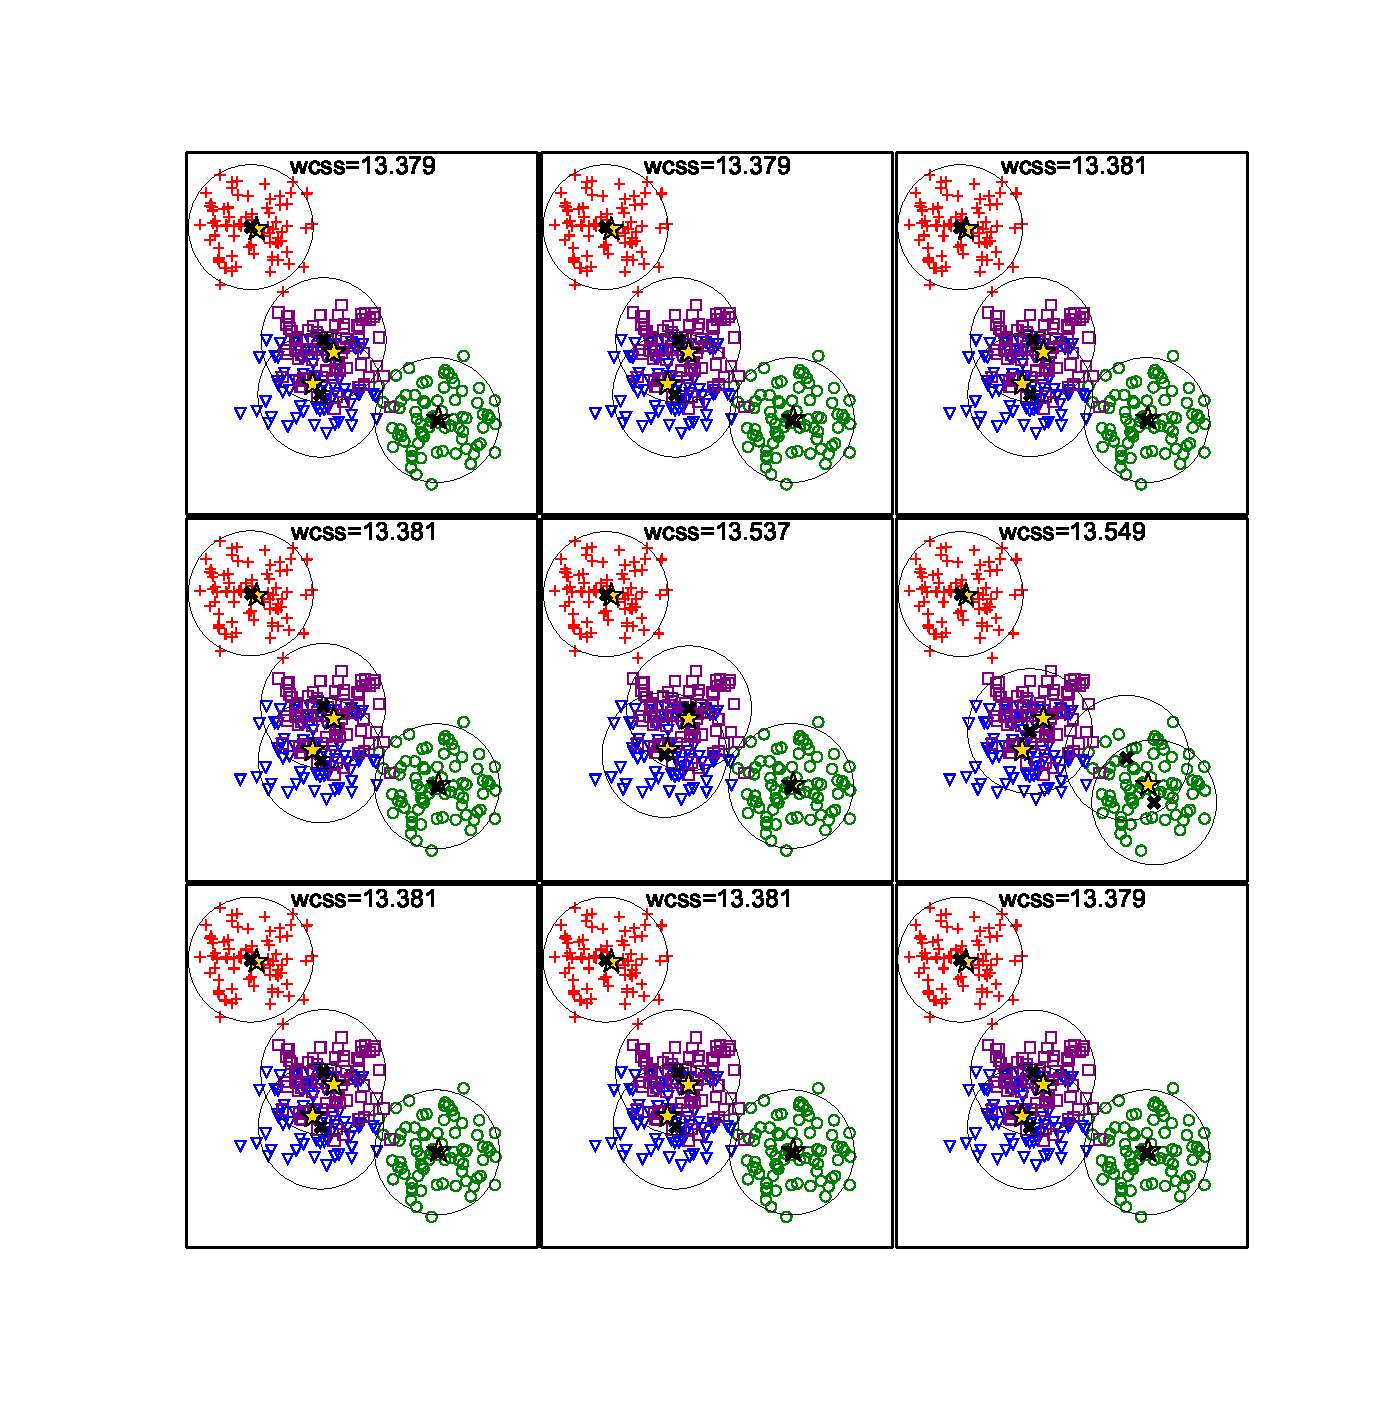
\includegraphics[width=1\textwidth]{figs/kmeanex}}
    \caption{Example $k$-means}{Example $k$-means on a dataset of 4 generated Gaussian clusters.  Gold stars mark the ground truth, and
      cluster symbol and coloring correspond to the vector's true membership.  Black X's mark the $k$-mean centroid
      estimates. The within-cluster sum of squares (WCSSE) is provided at the top of each plot.}\label{kmex}
\end{figure}

For points on a line, the $k$-means problem can be solved exactly in polynomial time using dynamic programming
techniques.  Unfortunately, this is a special case, and there is no known polynomial time algorithm for optimizing the
$k$-means criterion for generalized $\mathbb{R}^d$.  Following, if P$\neq$NP, optimizing the $k$-means heuristic is
Max-SNP/APX hard \cite{dasgupta08,Mahajan09}.  The two classes Max-SNP and APX are subsets of the NP class that deal
specifically with graph theoretic problems, and approximate optimization problems respectively.  These problems 
often have solutions that are can solve real world problems in polynomial(P) time, but are none-the-less in NP
for adversarially crafted problems.
Despite this somewhat dire outlook, APX problems such as $k$-means have
polynomial time bounded approximate solutions.  $k$-means not withstanding, $1+\epsilon$-approximate $k$-means can be
solved in linear time \cite{kumar}.  Furthermore, even simpler Lloyd-type algorithms tend to converge quickly on many
real-world datasets \cite{Jain}.

\section{Distributed Data}
Given the success of $k$-means algorithms and their relatively well behaved run time complexities, what need do we have
for another clustering algorithm?  While incremental algorithmic improvements result in shorter run-times they do not
often attack the fundamental issue of $k$-means's distributed scalability.  For this reason we propose an algorithm
that is specifically designed to overcome this issue that forestalls the communication requirement until the final
processing step.

\subsection{Distributed $k$-means}
A principal occupation of parallel computing research is speedup and the desire for a linear, or sub-quadratic
scaling.  Parallel speedup is the ratio of single compute node processing time versus parallel processing time or
$Speedup = T_s/T_p(n)$ , where $T_s$ is the time to process on a single node and $T_p(n)$ is the time to process in
parallel on $n$ compute nodes.  Of particular interest, is the shape of the ratio curve as $n\rightarrow \infty$, which
often is embedded in the underlying algorithmic structure.  The structure of the most common Lloyd-step $k$-means
clustering algorithm iteratively alternates between two steps, consisting of an assignment step followed by an update
step.  The assignment step, where centroids are assigned to their nearest representative cluster, can be made parallel by
processing data vector assignments in parallel.  However the update step, in which the cluster centroid is computed and
distributed to processors for the following assignment round, seems to be inherently sequential.  In distributed processing 
this issue is referred to as a sequential bottleneck or barrier synchronization.  Amdahl's Law gives the optimal speedup 
potential for parallel processing based on this ratio of required sequential $(s)$ code to parallel $(p)$ code.  More formally:
\begin{Theorem}[Amdahl's Law]
$$Speedup = {{1}\over{ (1-p)+{{p}\over{s}}}}.$$
\end{Theorem}

\begin{figure}
    \centerline{\includegraphics[width=.8\textwidth]{figs/speedup}}
    \caption{Amdahl's Law Speedup}{Amdahl's Law optimal Theoretical Speedup In a contention-less shared memory system for various
    parallel to total code implementations as a function of compute nodes}\label{aspeedups}
\end{figure}

In the case of Lloyd-step, $k$-means we can view the vector assignment step as parallel and the new centroid computation
as a sequential step.  Although this is perhaps an oversimplification, as centroid computation could also be
parallelized, Amdahl's Law speedup assumes contention-less accesses to shared memory, which does not exist in practice
as the number of processing nodes grows.  Instead additional communication overhead would be required, making the
centroid processing step sequential at best.  In Figure \ref{aspeedups} optimal speedups are shown for various ratios of
parallel to total code.

As discussed, even optimizing sequential to parallel code, will not overcome requirements due to network latency, 
memory contention and cache conflicts.  For these reasons,  recent work has focused on creating clustering
algorithms with lower communication overhead and fewer sequential bottlenecks. 

\subsection{Streaming Data}
In addition to being poorly suited for distributed analysis on static data, the standard $k$-means is not 
directly applicable to processing a continuous data stream. This is because, standard $k$-means requires a
pass through all of the data, to compute the final cluster centroids.  A requirement that is not available
in the streaming models. Next we define the streaming data model, its specific attributes and requirements.
In particular, the unbounded nature of the stream, implies that passing over all of the data, is not an option
for a streaming algorithm.
\begin{Definition}[Data Stream]
A data stream $S$ is a sequence of data vectors $v_1,v_2,...v_n \in V $ that arrive sequentially in time $t$ where
$t(v_1) < t(v_2) < ... < t(v_n) \forall v_i$, and the number of vectors $n$, is potentially 
unbounded ($n\rightarrow \infty$).  Each vector $v$ is of constant length, or is a variable length decomposable to 
constant length vector (e.g. words in sentences embedded in a sparse dictionary space).
\end{Definition}

Figure \ref{strmodel} provides an overview of the data stream model along with common attributes of many streaming
algorithms.  Data streams present a variety of challenges in both computational and storage complexity to clustering
algorithms.  The iterative nature of $k$-means requires that an entire dataset be accessible at any point in time.  Data
streams, however are potentially unbounded sequence of observations, with irregular arrival times.  Due to the unbounded
nature of streaming data, the entire set of vectors cannot realistically be stored in main memory.

\begin{figure}
    \centerline{\includegraphics[width=.8\textwidth]{figs/Streaming}}
    \caption{Streaming Model}\label{strmodel}
\end{figure}

In general there are three requirements that we regard as essential for streaming algorithms with $n$ observations, 
namely:
\begin{itemize}
 \item \textbf{Bounded Memory:} Due to the constraints of memory bandwidth in real machines, memory access patterns for
   data streams must be sequential allowing for one or a very small constant number of passes over the data.  The bound
   on the stored data, is sub-linear, and is usually regarded as either a predefined constant based on memory
   availability or $\theta(log(n))$.
 \item \textbf{Sub-Quadratic Processing Time:} Because the data stream is unbounded, it is infeasible to have an algorithm
   whose complexity is greater than $\theta(nlog(n))$ in regard to processing the entire data stream.  Or for each
   vector, no more than some constant$*log(n)$ steps may be performed.
 \item \textbf{Off-line-Step Complexity:} Due to the unbounded nature of the data stream, there is no reasonable start
   and end to the data stream.  As such, a streaming algorithm must be able to produce a result at any time throughout
   the evolution of the data stream, and in a reasonable amount of time.  While this amount of time is not strict, it
   invariably may only operate on the stored $\theta(log(n))$ data.
\end{itemize}

\noindent
In addition to the machine constraints presented by the streaming data model, streaming data often provides meaningful
temporal aspects.  One such attribute is changing trends over time.  Such trends as concept drift, occur often in the
semantic data space, and are a specific form of re-baselining in many other fields.  For this reason the concept of the
data stream, and subsequent clustering problems have been proposed \cite{silva-13} to capture these latent features.

\section{Sketching}

Following the requirements of streaming algorithms to have a bounded memory footprint, as with many big data problems in
computing accuracy is traded for memory.  One such method of lossy compression is the sketch data structure. The goal of
a sketch is to maintain an approximate record of the salient features of a dataset while not requiring that the entire
dataset be stored in main memory.  Sketch data structures have seen recent resurgence following the success of the
frequent directions algorithm \cite{libertyfreq}, hyperloglog \cite{hyperloglog}, counting \cite{cormode}, precision
sampling, and solutions to the $k$-Heavy-Hitters problem \cite{berinde}.

Sketching tends to offer one of two trade offs for memory, either lossy and sampling methods which older elements
ignored or forgotten or space saving, in which elements sketches lose accuracy over time.  \textsf{RPHash} resorts to the latter
exchange, and accept loss of accuracy over time.

\subsection{Count-Min Sketch}

One such data structure for space saving sketching is the Count-Min Sketch \cite{cormode}. The general idea is to
partition the element range into a finite set of discrete hash buckets, then update the bucket's value instead of
storing each element.  Due to the likelihood of hash collision in the element range, multiple copies with different hash
functions from the same family are updated in parallel.  To query an item's sketched value, all bucket sets are
searched, and the minimum of the searched buckets is returned.  The result of the minimum over multiple inaccurate
searches results in an amplification of accuracy for the searched element following, similar to minimum over chained
bloom filters.  Buckets update false positively often, but are never false negative for a given element, therefore the
minimum is the closest to the real count value.  Figure \ref{countmin} gives a diagram of this behavior for a toy
example.  Rigorous mathematical proof of the accuracy for this data structure has been studied in \cite{cormode3}.

For a positive only counter, the error in counting corresponds to the best of the $d$ approximate counts with error due
to noise from other counts, of $1/w$.  For $d$ hash functions if we chose $d = \log 1/\delta$ and $w=2/\varepsilon$ we
have an estimate for the count that is at most $\varepsilon N$ with probability greater than $1-\delta$.  Following a
proof in \cite{cormode2} using the Chernoff bound, the probability of returning a `bad' estimate is exponential in $d$.

\begin{figure}
    \centerline{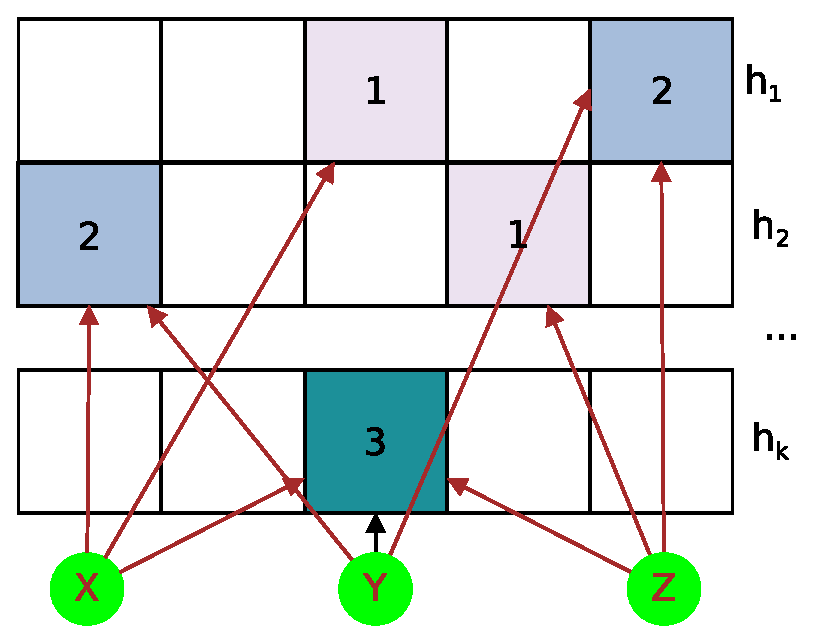
\includegraphics[width=.6\textwidth]{figs/countmin}}
    \caption{Count-Min Sketch}\label{countmin}
\end{figure}

\section{Dimensional Reduction}\label{rpprelim}

Dimensional Reduction is a key occupation for high dimensional data analysis.  Yet another face of the Curse of
Dimensionality, high dimensional data suffers from a loss of contrast between near and far points, making euclidean
metrics and even non-euclidean metrics useless as dimensionality grows.  This can be seen in the limit of the volume
occupied by a distance metric and an orthogonal space embedding approaching 0 as the embedding dimension grows.  Here we
give an informal proof of this approach.  The euclidean metric essentially carves out hyper-spheres in high dimensional
space as we can see from the distance function $d(x,y) = \sqrt{\Sigma(x_i-y_i)^2}$.  However, orthogonal embeddings with
many dimensions often distribute volume in coordinate space along rectangles.  We can see the ratio of the volumes of
these two geometric objects as dimensionality grows by taking the dimensional parameterization of the volume equation
for spheres and cubes with radius $r$ and side length $2r$.  Formally this derivation is

\begin{enumerate}\label{sphere2rect}
\item $ \text{Sphere\_Volume}(d) =  {{r^d\pi^{d/2}} \over {\Gamma(d/2+1)}}$
\item $\text{Cube\_Volume}(d) = 2r^d $
\item dropping constants, we get the asymptotic ratio:
$$
\mathlarger{\mathlarger{\theta}} \bigg({{\text{Cube\_Volume}} \over {\text{Sphere\_Volume}}}\bigg) =
{{(2r)^d \Gamma(d/2)} \over {\pi^{d/2}r^d}}
$$
\item replacing $\Gamma$  with Stirling's Approximation:
$$
= {   {  (2r)^d\sqrt{\pi d} ({{d}\over{2e}})^{d/2}   }\over {\pi^{d/2}r^d}  }
$$
\item dropping constants and simplifying:
$$
 = {{d^{d/2}(2/e)^{d/2}} \over {\pi^{d/2}}}
$$
\item taking the limit:
$$
\underset{d\rightarrow \infty} {\lim} { d^{d/2} \bigg({ {2}\over{e\pi}}\bigg)^{d/2}} = \infty.
$$
\end{enumerate}
\noindent
Even non-euclidean metrics exhibit this behavior.  This can be attributed to a more complicated analysis of the ratio of
the difference between the maximum distance and minimum distance divided by the maximum distance, often referred to as
contrast, approaching $0$ as $d\rightarrow \infty$.  A thorough investigation of this is given in \cite{zimek12,
  Aggarwal01, Beyer1999}

\subsection{Conventional Dimensional Reduction}
Conventional dimensional reduction techniques consist of the classic Principal Component Analysis (PCA) reduction which consists of
computing the directions of maximum variance in the data, and projecting the data along the a subset of vectors
corresponding to the greatest variance vectors.  PCA based reductions are useful and provide an embedding that optimizes
the error in the $L_2$-norm.  PCA reductions however require considerable computation, and are not suited for streaming
environments.  Frequent Directions \cite{libertyfreq} tend to mitigate these limitations but is are still fairly new in terms
of adoption.

Another technique for dimensional reduction is the t-SNE \cite{tsne} technique.  t-SNE is similar to PCA in its minimization
of an objective, however instead of minimizing the $L_2$-norm difference, it optimizes the Kullback-Leibler divergence.
Similarly it is not well suited for the streaming environment, as the minimization requires all data, and follows
a gradient descent approach to minimize the objective function.

\subsection{Random Projection}
Random projection is a method in which high-dimensional data vectors are projected down to a lower dimensional space by
applying a projection following some specifically crafted matrix.  One such example of an optimal distance preserving
projection would be the result of the truncated principal component projection.  Unfortunately PCA is computationally
complex and requires multiple scans over the entire input dataset.  However as the original embedding dimensionality
grows, the distortion between PCA projection and random projection tends to converge.  A random projection matrix is
composed of orthogonal vectors sampled from some random or quasi-random distribution.  Random projection can achieve a
bounded error distortion factor very close to the optimal $L_2$ norm subspace embedding that would otherwise result from
the principal component decomposition based projection \cite{bourgain1985lipschitz}.  The resurgence of the random
projection method of Johnson and Lindenstrauss was reinvigorated with the work of Achlioptas on Database Friendly
Projection that provided good subspace embeddings requiring minimal computation costs \cite{Achlioptas01}.

\subsection{JL Lemma}
The Johnson-Lindenstrauss Lemma defines the error bounds of random projection.  This formal bound for our projections
$f(\cdot)$ that preserves the distance between any two vectors $u$ and $u'$ with error $\epsilon$ is given as: 

\begin{Theorem}[Johnson-Lindenstrauss Lemma \cite{vempala}]
$$
 (1-\epsilon) \|u-u'\|^2 \leq \|f(u)-f(u')\|^2 \leq (1+\epsilon) \| u-u' \|^2
$$
\end{Theorem}

In Figure \ref{projex} results are given for a randomly generated dataset from $\mathbb{R}^{10000}$ of vectors that are
unit distance apart.  The vectors are randomly projected down to $\mathbb{R}^{10000}$, $\mathbb{R}^{1000}$,
$\mathbb{R}^{100}$, and $\mathbb{R}^{24}$ and the \textbf{L2} distance is calculated.  As the bound suggests, average
distance is consistently unit.  However, higher degrees of projection result in a greater occurrence of outliers and
overall increase in overall variance.

Under the optimal $\epsilon$-preserving mapping $f(\cdot)$, the Johnson-Lindenstrauss lemma results in a tight bound for
$u,u' \subseteq U$ and $n=|U|$, of $d \sim \Theta( {\frac{log(n)} {\varepsilon^2 log(1/\varepsilon) }})$.  The bound was
later applied to random orthogonal projections in Frankl and Maehara, and found to have a similar order on the bound for
the projected subspace dimensionality \cite{Frankl}.  Vempala gives a relaxation of the JL-bound for random orthogonal
projections, arriving at $d \sim \Omega(log(n))$ \cite{vempala}, with a scaling factor of ${\frac{1}{\sqrt{d}}}$ to
preserve approximate distances between projected vectors.
An additional benefit of using Random Projection for mean clustering is that randomly projected asymmetric clusters tend
to become more spherical in lower dimensional subspace representations \cite{bingham}.  Mean and medoid clustering
algorithms, such as \textsf{RPHash}, are predisposed to spherical clusters.

\begin{figure}
    \centerline{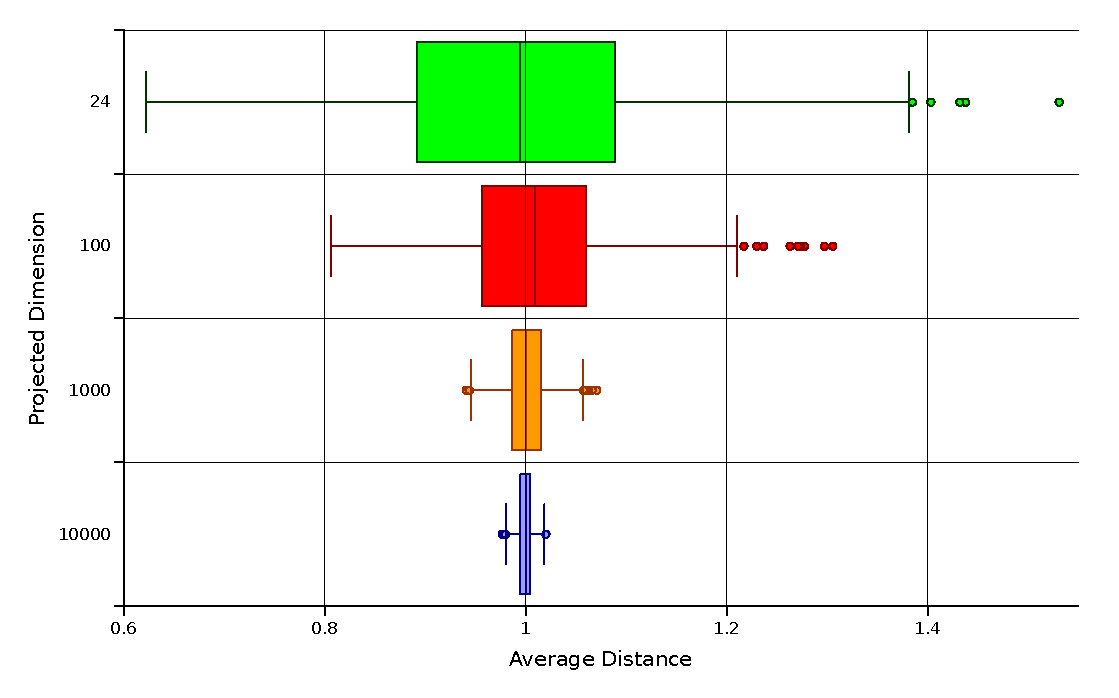
\includegraphics[width=.9\textwidth]{figs/projectiondimensionVSaveragedistance}}
    \caption[Experiment with Random Projection and Distance]{Example random projection dimension and expectation of distances for vectors that are unit distance
      apart.}\label{projex} 
\end{figure}

\subsection{DB-Friendly Projection}
Using the intuition that the dot product with a vector composed of zero mean Gaussian random variates, amounts to a
great deal of multiplication by values near zero, D. Achlioptas describe a far more efficient projection matrix with
surprisingly more favorable attributes than multiplication by a dense Gaussian matrix \cite{Achlioptas01}.  
These so-called DB-Friendly projections provide dimensional reduction that adheres to the JL-Bound, and in many cases
provide lower error embeddings than the more computationally intensive Gaussian matrix projection \cite{Achlioptas01}. 
Computed efficiently, the DB-Friendly Projection method requires $\theta(dm/3 )$ steps.
The DB friendly matrix is constructed as: $r_{ij}\in\textbf{R}$ is $m\times d$ as follows:
\[
    r_{ij}= \sqrt{1/d}
\begin{cases}
    +1, & \text{with probability } {\frac{1}{6}}\\
     0, & \text{with probability } {\frac{2}{3}}\\
    -1, & \text{with probability } {\frac{1}{6}}\\
\end{cases}\text{\cite{Achlioptas01}}
\]

\subsection{Fast Johnson Lindenstrauss Transforms (FJLT)}

Advances in compressed sensing and Restricted Isometry Property (RIP) have pushed the bounds of random projection to
nearly optimal and work efficient samplings of the input data following a realization that the underlying goal of random
projection is to evenly represent a mixture of the input space vectors.  To optimize this mixture, FJLT looks to the
Heisenberg principle in harmonic analysis, stating that the spectrum and signal cannot both be
concentrated \cite{ailon2006}.  The FJLT consists of a projection matrix product $\Phi = PHD$ that consists of two random
matrices, $P$ a sparse $m\times d$ Gaussian, $D$ a $m\times m$ diagonal ``coin-flip'' matrix, and $H$, the rank $m$
Hadamard matrix.  The resulting matrix projection requires only $\theta(m \log m)$ time where $m$ is the original
dimension.

\section{Space Quantization} 
Switching from the continuous spaces of random projections, we now consider the discrete space partitions induced by
lattices.  Optimal implementations of grid based clustering algorithms such as DBSCAN \cite{dbscan} and DStream \cite{cao-06}, require
that the data space be partitioned as evenly as possible.  Furthermore to avoid costly interprocess communication
overhead, a universally generative naming scheme must be established.  For known datasets, a perfect partition of the
data space can be produced by the Voronoi diagram \cite{Klein1988}.  In 2-dimensional space, Voronoi Diagrams can be
generated in $\Theta(n log(n))$-time \cite{Fortune}.  However, higher dimensional algorithms for Voronoi partitioning
have far less favorable runtime complexities \cite{Gavrilova2003}, making them inefficient for partitioning arbitrarily
high dimensions.
A solution to this partitioning problem is to sacrifice the optimal partitioning and accept a probabilistically  
close partitioning.  Such is the case with Locality Sensitive Hash (LSH) functions. 
LSH functions use collision probability dependent on distance to chain regular partitionings together to
approximate optimal partitions. Now we present a formal definition for LSH. 
\begin{Definition}[Locality Sensitive Hash Function \cite{datar-04}]
let $\mathbb{H}=\{h:S \rightarrow U\}$ is $(r_1,r_2,p_1,p_2)-$sensitive if for 
any $u,v\in S$
 \begin{enumerate}
   \item if $d(u,v) \leq r_1$ then $Pr_{\mathbb{H}}[h(u)=h(v)]\geq p_1$
   \item if $d(u,v) > r_2$ then $Pr_{\mathbb{H}}[h(u)=h(v)]\leq p_2$
 \end{enumerate}
\end{Definition}

Lattices, are an alternative, mathematical structure, that can partition infinite, fixed dimensional data spaces in a
generative way. We give an example of the $A_2$ Lattice in Figure \ref{lshex}.  Furthermore, lattices formed from binary codes (such as $E_8$ and Leech Lattice) have extremely
efficient nearest neighbor decoding algorithms.  A formal definition of a lattice constructed from a linear code is:
\begin{Definition}[Lattice in $\mathbb{R}^n$ \cite{Pless}]\label{latticedef}
let $v_1, ...  , v_n$ be $n$ linear independent vectors where $v_i=v_{i,1}, v_{i,2}, ...
,v_{i,n}$.  The lattice $\Lambda$ with basis $\{v_1, ...  , v_n\}$ is the set of all
integer combinations of $v_1, ...  , v_n$ the integer combinations of the basis vectors
are the points of the lattice.
$$\Lambda = \{z_1v_1+z_2v_2+ ...  +z_nv_n | z_i\in \mathbb{Z}, 1 \leq i \leq n\}$$ 
\end{Definition}

\begin{figure}
    \centerline{\includegraphics[width=.4\textwidth]{figs/2dLat}}
    \caption{$A_2$ Lattice Constellation}\label{lshex}
\end{figure}

\subsection{$E_8$ Lattice Decoder}

The $E_8$ Lattice or Gosset's Lattice provides an optimal sphere packing in 8 dimensions.  Furthermore, the nearest
neighbor decoding complexity of $E_8$ is relatively low, owing to its decomposition into $E_8 = D_8 \cup
<{1\over2}>+D_8$.  $D_8$ decoding entails a simple rounding technique among the vectors in $\mathbb{R}^8$ and an overall
parity check.  Further advancements \cite{SPLAG} in the decoding complexity of $E_8$ result in a decoder requiring only
72 steps.  However, due to $E_8$'s relatively low dimensionality, we must also apply a rudimentary outer decoding step
which simply splits a projected vector of dimension higher than 8 into multiple $E_8$ decodings.

\subsection{Leech Lattice Decoder}

The Leech Lattice is a unique 24 dimensional lattice with many exceptional properties \cite{Curtis,SPLAG}.  Of
particular interest to this work is the Leech Lattice's packing efficiency.  The Leech Lattice defines an optimal
regular sphere packing of 24 dimensional space \cite{leech} and serves nicely as a space quantizer for
\textsf{RPHash}.  Furthermore, the Leech Lattice, being the cornerstone of many intriguing mathematical
concepts, has various relationships with other sub-lattices that offer useful algorithmic decompositions.

Among some of the most efficient decoders for the Leech Lattice, Amrani and Be'ery's \cite{Amrani} decoder has a
worse-case decoding of only 331 floating point operations.  Although higher dimensional lattices with comparable packing
efficiency exist, the decoding complexity, in general, scales exponentially with dimension \cite{Tarokh1,Agrell}.

\subsection{Spherical Locality-Sensitive Hashing}

Another method of space partitioning applicable to data where the vector norm is 1, or rather lies on the surface of a
hypersphere, is the Spherical LSH technique of Terasawa \cite{SLSH}.  Spherical LSH uses an inscribed regular polytope
to partition the surface of the sphere where vertexes of the polytope correspond to partition regions.  Although other
regular d-polytopes such as the d-simplex and d-hypercube exist, we focus on the d-orthoplex, following the favorable
collision probability per distance, which results in Table 1 of \cite{SLSH}.  The $d$-orthoplex is a regular d-polytope
with $2d$ vertexes corresponding to the positive and negative axis per dimension of a $0$ centered unit hypersphere
embedding.  The nearest vertexes can be searched among the $2d$ vertexes following the max dot product method given in
\cite{SLSH}, resulting in a search time complexity of $\theta (d^2)$.  The $d$-orthoplex has the benefit over $E_8$ and
Leech Lattice decoders of allowing for arbitrary projection dimensions, with the disadvantage that it is only strictly
applicable to vectors lying on the surface of a hypersphere.

\subsection{Collision of LSH Functions}
As stated above, a desired trait of an LSH function is a discriminative collision probability curve with respect to
inter-point distance.  In Figure \ref{prcollision} we give the collision probability curve for set of LSH
functions: The Leech Lattice($\Lambda_{24}$), Multi-$E_8$, Spherical LSH (SLSH), and the Gaussian $p$-Stable distribution.  
Notable, multi-$E_8$ gives the tightest overall curve, with $\lambda_{24}$ following closely in terms of discrepancy ratio
for distance $p = {{r_1} \over {r_2}}$.

\begin{figure}
    \centerline{\includegraphics[width=.8\textwidth]{figs/prcollisions}}
    \caption{Probability of collision as a function of distance for various decoders for vectors in
      $\mathbb{R}^{24}$}\label{prcollision} 
\end{figure}

\section{Differential Privacy}

Security is another issue that arises in the distributed clustering problem.  Medical, financial, and proprietary
commercial data are often targets for clustering that have security requirements not addressed in the local clustering
setting.  Data privacy is often important in machine learning due to the sometimes sensitive nature of records in a
dataset.  Distributed and streaming data analysis applications have additional security requirements due to the
sometimes insecure transport mechanisms between processing nodes.  The cryptographic concept, differential privacy,
provides some solutions to these problems.  The result is often a trade-off between privacy and data loss or additional
processing requirements.  This general concept is referred to as Differential Privacy \cite{diffpriv}.

\subsection{$k$-anonymity}

$k$-anonymity is privacy technique that defines a number $k$ of records that are equivalent based on the record's
attributes.  Generalization and suppression are employed, such that data utility is not lost, and the $k$-anonymity
constraint is met for some $k$ \cite{Aggarwal2008}.  An intuitive example would consist of a set of patient records with
various attributes.  One such attribute could be age, employing the rounding technique, one could coerce two records to
being equivalent, by changing the exact age to a range of ages such as 18-25, instead of 19, and 23.  Such a obfuscated
dataset would have $k=2$ -anonymity.

\subsection{$l$-diversity}

An extension of $k$-anonymity, $l$-diversity attempts to protect the attributes as well as the records.  $l$-diversity
overcomes some of the flaws in $k$-anonymity, by requiring that a dataset has at least $l$ different values for each
attribute.  Common ways to achieve $l$-diversity are random sampling and additive noise.

\section{MapReduce}
MapReduce \cite{dean-08} and similar programming structures have become popular in recent years with the so called big data revolution.
These architectures abstracted out the often tedious and difficult management tasks of maintaining a fault tolerant,
distributed, processing system.  Furthermore, they made heterogeneous computing on commodity hardware the norm for big
data processing that it is today.  This change allowed more people and businesses to take advantage of large scale
processing while not requiring specialized hardware or in the case of Platform as a Service (PaaS) architectures removed
the need for hardware altogether.

MapReduce is a distributed processing framework in which the focus is data locality facilitated by a functional
programming approach.  Common to functional programing, the Map and Reduce functions perform specific operations on data
instead of the data-flow approach in which data is distributed to processors.  The map function is an operation that
maps data to a discrete set of keys, while the reduction function aggregate the keys.  From the distributed computing
context this process scales well so long as the key-set and reduced data are not exceedingly large compared to the
original data.  By strictly adhering to Map and Reduce functions, data can be distributed horizontally across a set of
systems during the data collection phase, and small data bandwidth operations can be broadcast (scatter) to be performed
on the processing node's local data.  The key reduction step is also optimized in this framework, as key aggregation can
be performed on a peer-to-peer basis (gather).  While these processing method are not new, perhaps the more long lasting
result is the proliferation of freely available distributed processing frameworks.

\begin{figure}
    \centerline{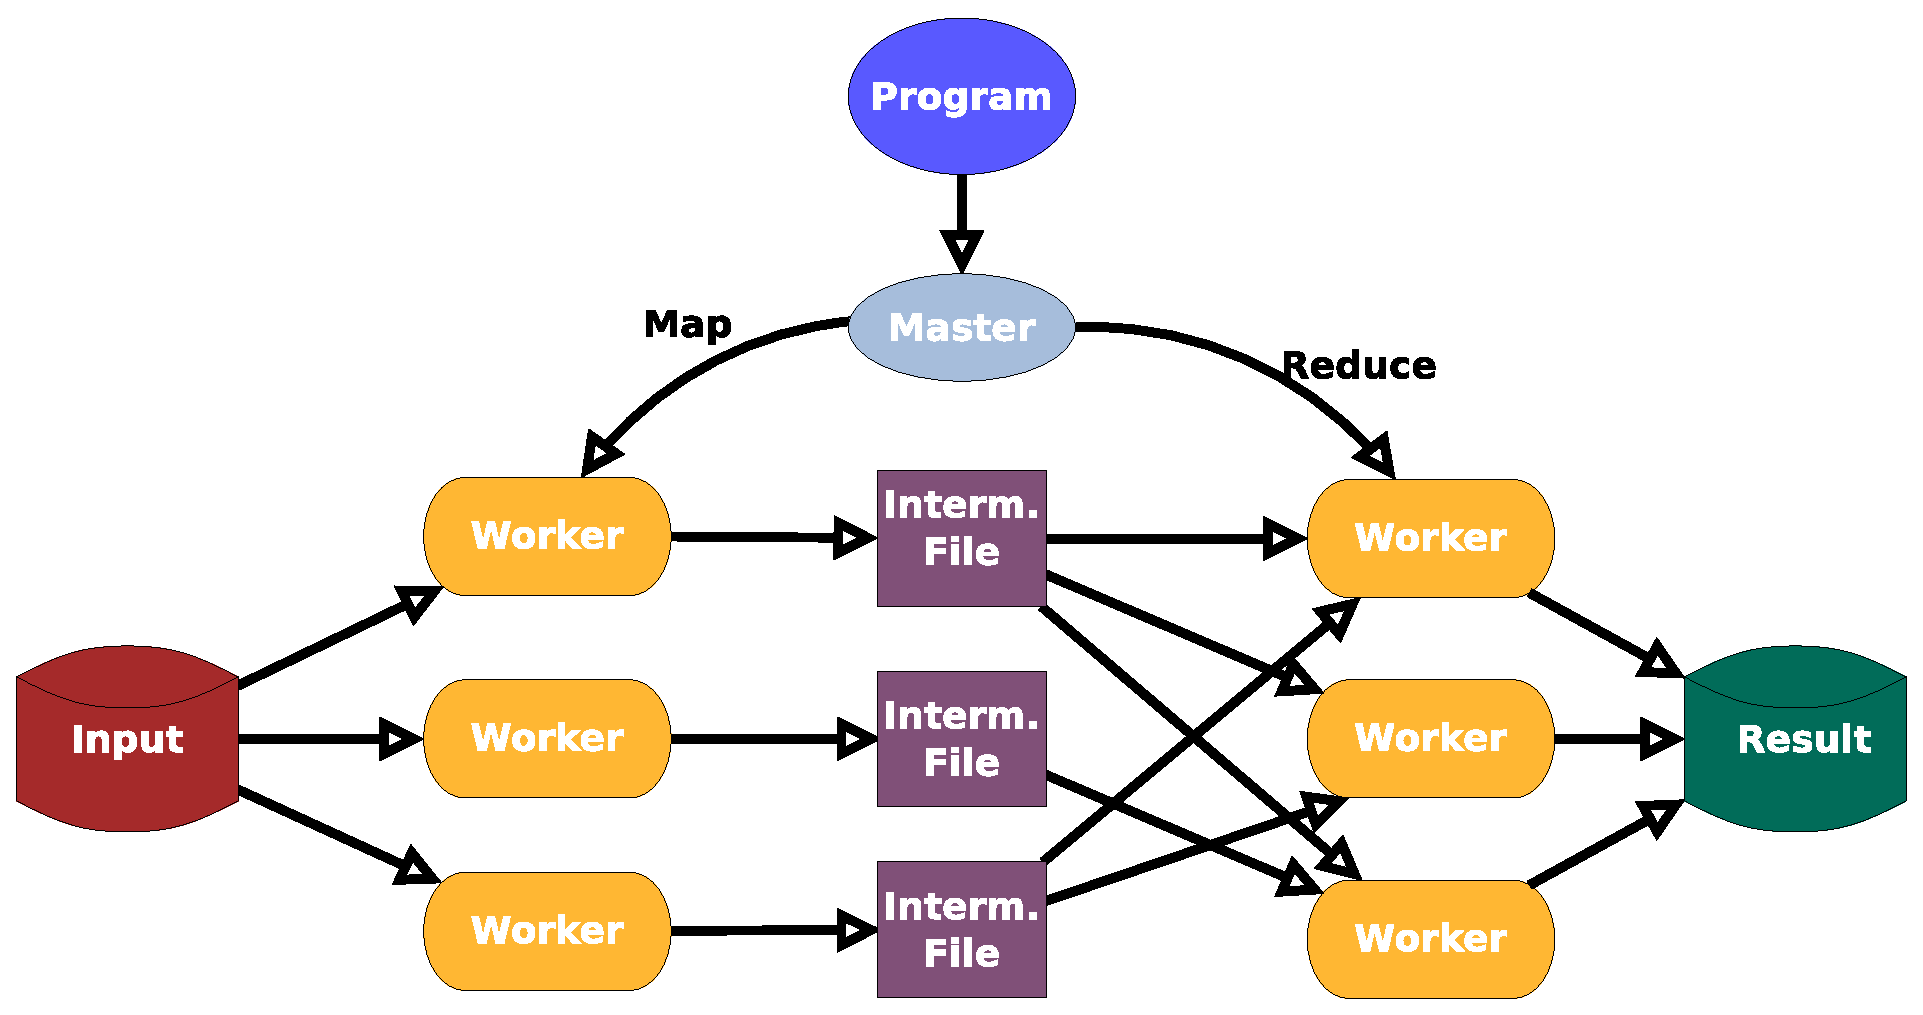
\includegraphics[width=.8\textwidth]{figs/mapreduce}}
    \caption{Map Reduce Step}\label{mr}
\end{figure}

Hadoop from the Apache Foundation is a popular version of the map-reduce framework written in Java.  Hadoop also includes a 
distributed file system (HDFS \cite{shvachko-10}) as well as monitoring tools, and extensions various computing tasks such as machine learning,
namely the Mahout package.

Spark \cite{chowdhury-10,zaharia-10} is an extension of map reduce that performs in memory data manipulation while also allowing for more flexibility
in the processing sequence.  In standard map-reduce, only a single shot, map (read from disk) and reduce (write to disk)
operations are preformed.  Various meta-frameworks have mapped the map-reduce task, however they strongly incurred the
disk IO processing bottleneck.  Spark continues the functional approach to distributed processing, namely map and
reduce, but extends it to utilize in memory storage and multiple applications of map and reduce.  In addition to
supporting a more generic map-reduce distribution, Spark also support streaming data processing.  Streaming data
processing consists of a continuous stream of data distributed to processing nodes, with periodic `off-line'
synchronization processes.  Figure \ref{strmodel} depicts a point in time in the streaming model with earlier and past
time represented by a darkening of the data stream squares.  In this work it is adequate to interpret each block as not
necessarily uniform sized, batch of data vectors evolving over time.  For each batch of vectors, a sub-linear sketch of
the data is updated.  Periodically or at the request of a user, the sketch can be analyzed by an `off-line' step that
yields a result given the current state of the data stream.  In the case of a clustering algorithm this would be a set
of centroids.  We refer the reader to Silva \cite{silva-13} and Aggarwal \cite{Aggarwal2007} for an extensive analysis
and definition of various goals and methods in data stream clustering.  In this work we will focus on finding fixed $k$
non-moving centroids.
